%by AnMnv

\documentclass[14pt,a4paper]{scrartcl}
\usepackage[left=1.5cm,right=1.5cm,
    top=1.5cm,bottom=1.5cm,bindingoffset=0cm]{geometry}

\usepackage[T1,T2A]{fontenc}
\usepackage[utf8]{inputenc}
\usepackage[english,russian,ukrainian]{babel}
\usepackage{tabularx}
\usepackage{amssymb}
\usepackage{color}
\usepackage{amsmath}
\usepackage{mathrsfs}
\usepackage{listings}
\usepackage{graphicx}
\graphicspath{ {./images/} }
%\usepackage{draftwatermark} не будет лезть на картинки
\usepackage[printwatermark]{xwatermark}%будет лезть на картинки
\usepackage{lipsum}
\usepackage{xcolor}
\usepackage{tikz}
\definecolor{lgreen}{rgb}{0.5,1,1}]
\definecolor{n}{rgb}{1,0.5,0.5}
\definecolor{n1}{rgb}{1,1,0.5}
\definecolor{n3}{rgb}{1,0.7,0.9}
 \usepackage{csvsimple}
 \usepackage{supertabular}
\usepackage{pdflscape}



\begin{document}
\pagestyle{plain}
\pagecolor{white}






\begin{titlepage}
  \begin{center}
    \large
    Національний технічний університет України \\ "Київський політехнічний інститут імені Ігоря Сікорського"


    Факультет Електроніки

    Кафедра мікроелектроніки
    \vfill

    \textsc{ЗВІТ}\\

    {\Large Про виконання розрахункової роботи №1\\
      з дисципліни: «Теорія поля»\\[1cm]

   % ДОСЛІДЖЕННЯ ВИПРЯМЛЯЮЧИХ НАПІВПРОВІДНИКОВИХ ДІОДІВ\\

    }
  \bigskip
\end{center}
\vfill

\newlength{\ML}
\settowidth{\ML}{«\underline{\hspace{0.4cm}}» \underline{\hspace{2cm}}}
\hfill
\begin{minipage}{1\textwidth}
Виконавець:\\
Студент 3-го курсу \hspace{4cm} $\underset{\text{(підпис)}}{\underline{\hspace{0.2\textwidth}}}$  \hspace{1cm}А.\,С.~Мнацаканов\\
\vspace{1cm}

Превірила: \hspace{6.1cm} $\underset{\text{(підпис)}}{\underline{\hspace{0.2\textwidth}}}$  \hspace{1cm}Т.\,А.~Саурова\\

\end{minipage}

\vfill

\begin{center}
2020
\end{center}
\end{titlepage}




\begin{center}
\textbf{ЗАВДАННЯ} \\
\end{center}

\textbf{1.} Розрахувати розподіл потенціалу в міжелектродному просторі польового транзистора (варіант конструкції вибирається за передостанньою цифрою номера залікової книжки) з точністю до 0,01 В. Номер варіанту обирається за останньою цифрою номера залікової книжки.\par

\textbf{2.} Побудувати картини поля за допомогою еквіпотенціалей і векторів напруженості електричного поля. Побудувати косокутну проекцію потенціального рельєфу U(x,y) = $-e\cdot V(x,y)$\\
\begin{figure}[h]
\center{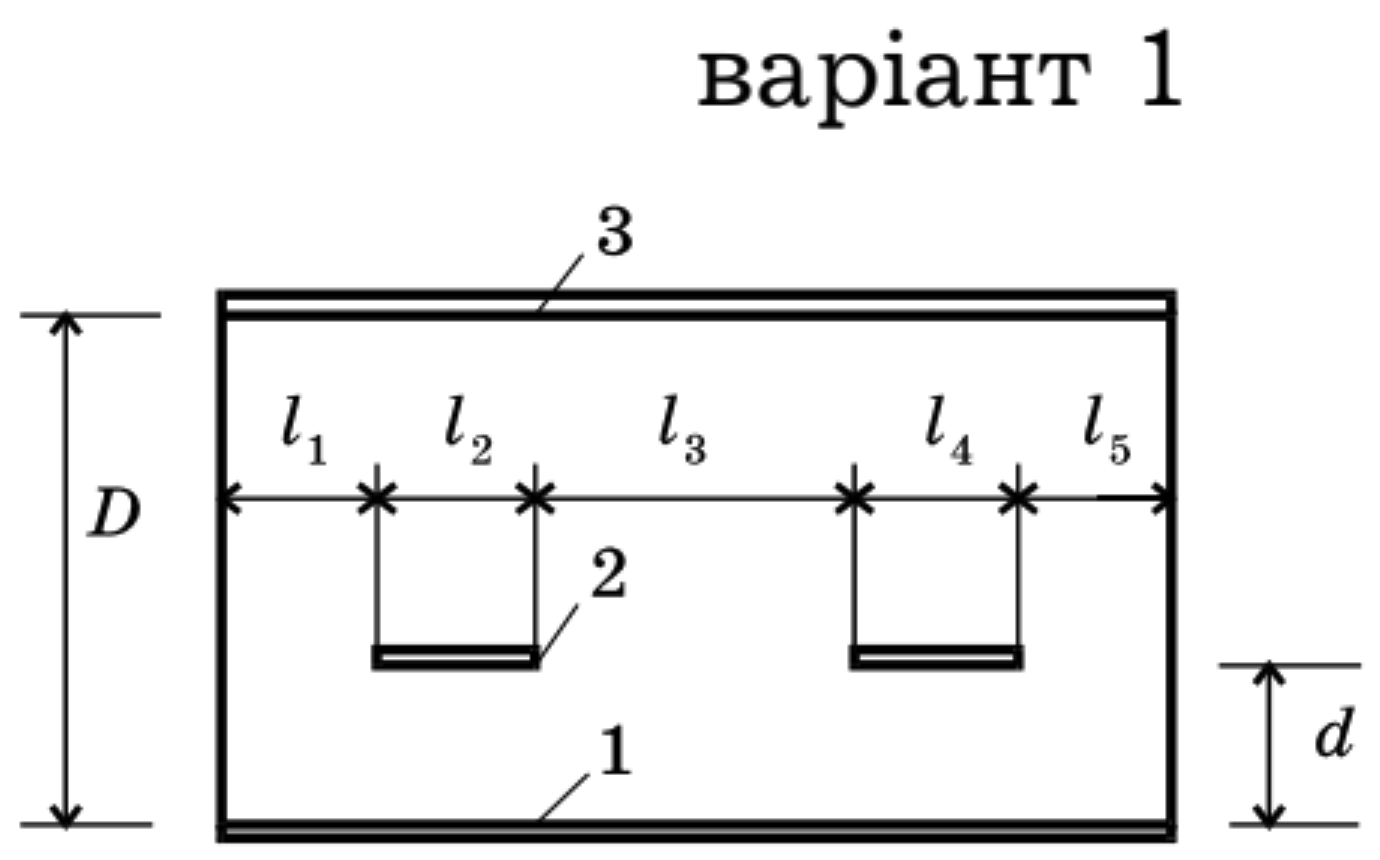
\includegraphics[width=0.5\linewidth]{var1.png} \\
$ l_1 = l2 = l_3/2 = l_4 = l_5 = 1,0$ мкм, d = 1,0 мкм,\\ D = 3,0 мкм 1 – витік, 2 – затвор, 3 – стік }
\end{figure}

\begin{center}
\vspace{0.1cm}
\begin{Large}
\begin{tabular}{ | c |  c |  c |  c |}
\hline
вар. № & 4   \\
\hline
$-V_{3B},B$ & 0.5   \\
\hline
$V_{CB}, B$ & 3   \\
\hline
\end{tabular}
\end{Large}
\vspace{0.2cm}
\end{center}

\newpage
\begin{center}
\textbf{РОЗРАХУНКИ} \\
\end{center}

Одним з найбільш розповсюджених методів розрахунку розподілу потенціалу в міжелектродному просторі польового транзистора є мотод скінченних різниць. В основу методу покладена заміна похідних в рівняніі Лапласа малими приростами. Розглянемо його для плоского поля V (x, y). Надаючи по черзі аргументам x і y деякої неперервної функції V (x, y) малого приросту з кроком h, можна приблизно (з точністю до величин другого порядка малості відносно
 $h^2$) замінити приватні похідні функцііотношеніямі різниць рис.\ref{ris:image5} :

\begin{center}
\begin{figure}[h]
\center{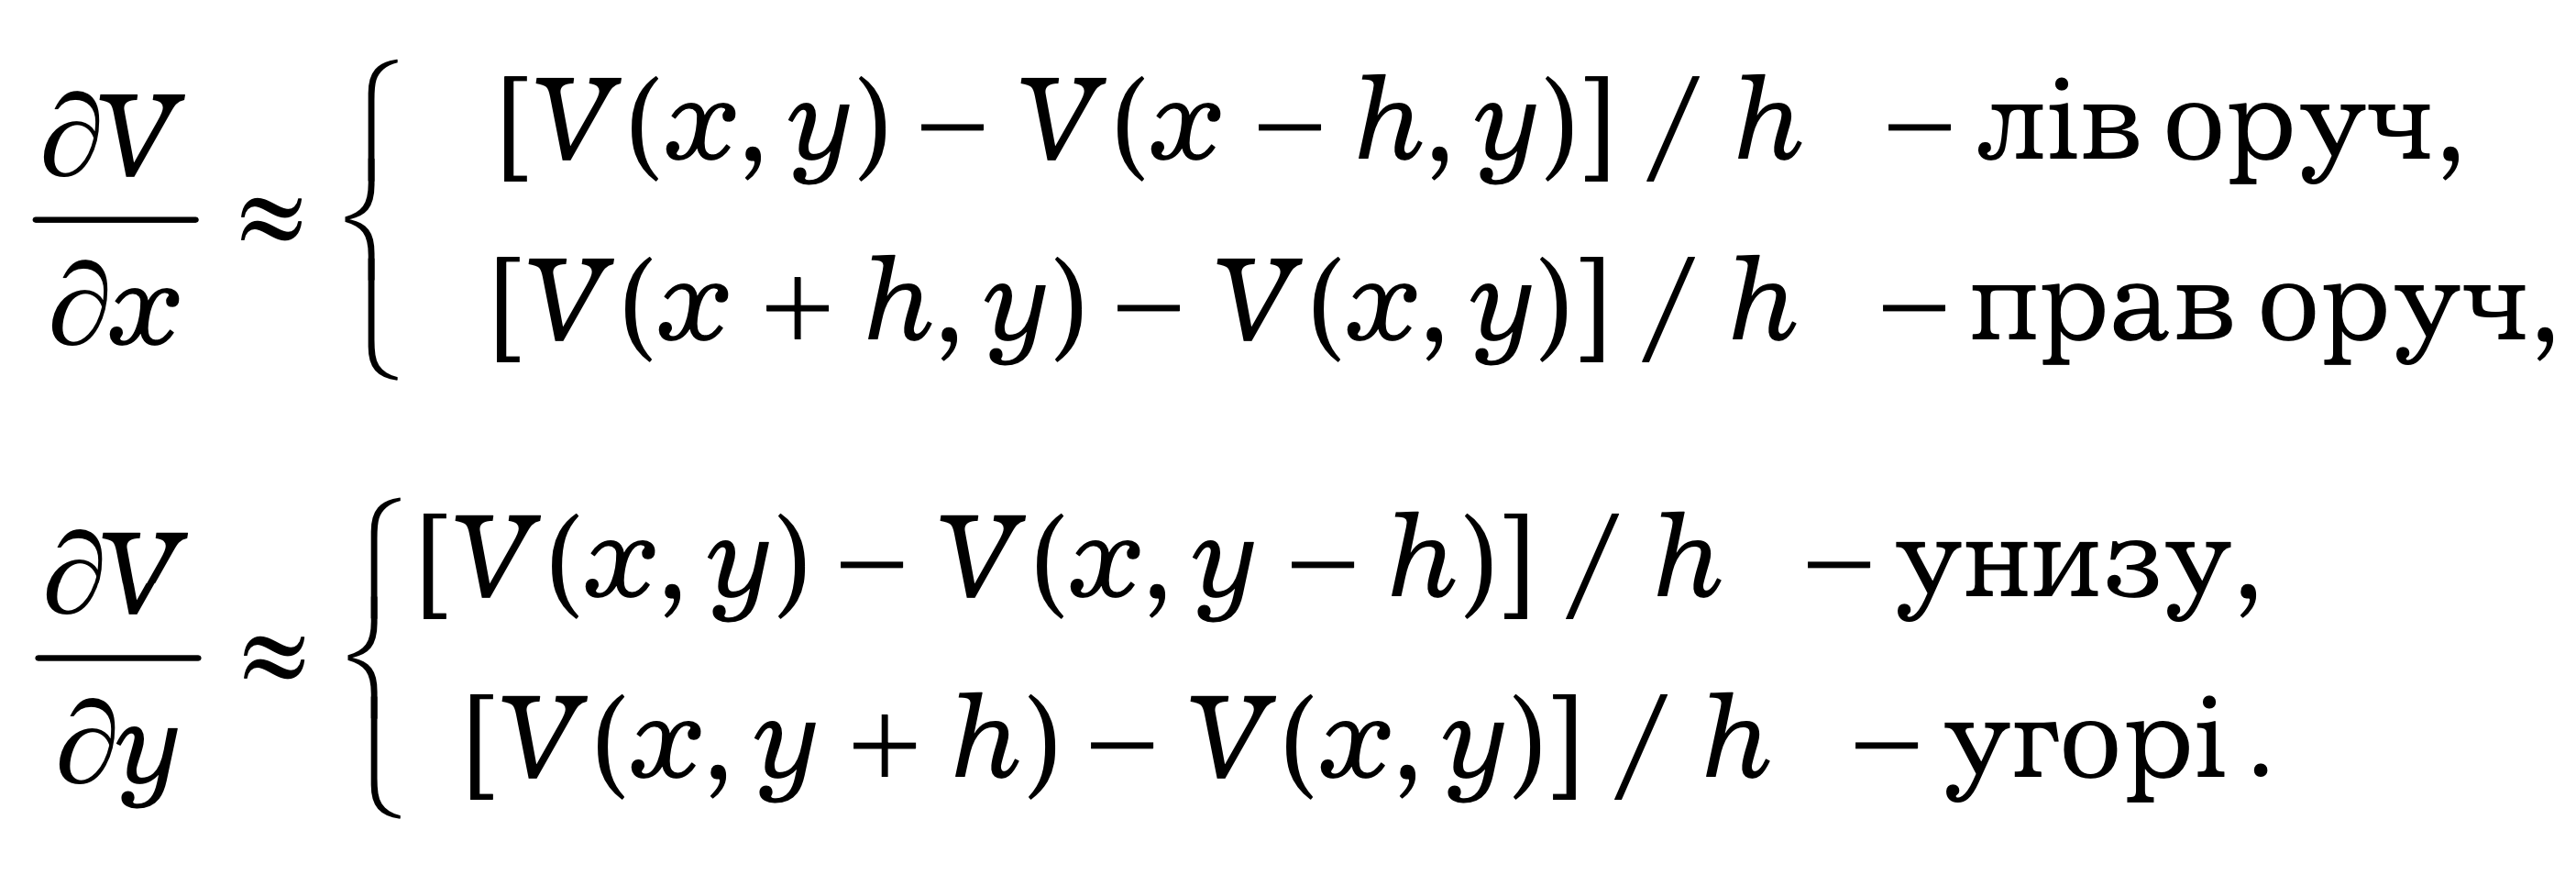
\includegraphics[height=4cm, width=12cm]{f.png}}
\end{figure}
\end{center}

\begin{center}
\begin{figure}[h]
\center{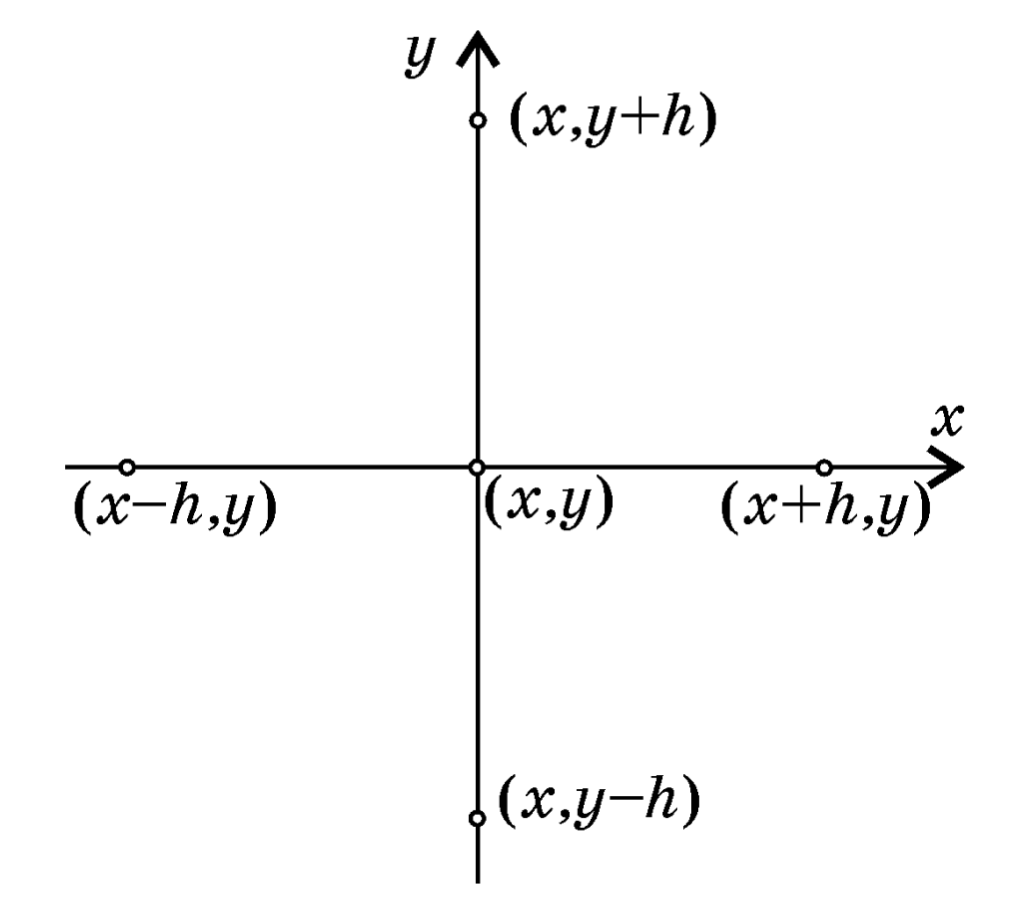
\includegraphics[height=8cm, width=8cm]{5t.png}}
\caption{П'ятиточкова схема для обчислення похідних через кінцеві прирости і розрахунку потенціалів..}
\label{ris:image5}
\end{figure}
\end{center}

\newpage
Представимо всю площину транзистора як  дискретний масив точок розмірністю 25х13.

\begin{center}
\begin{figure}[h]
\center{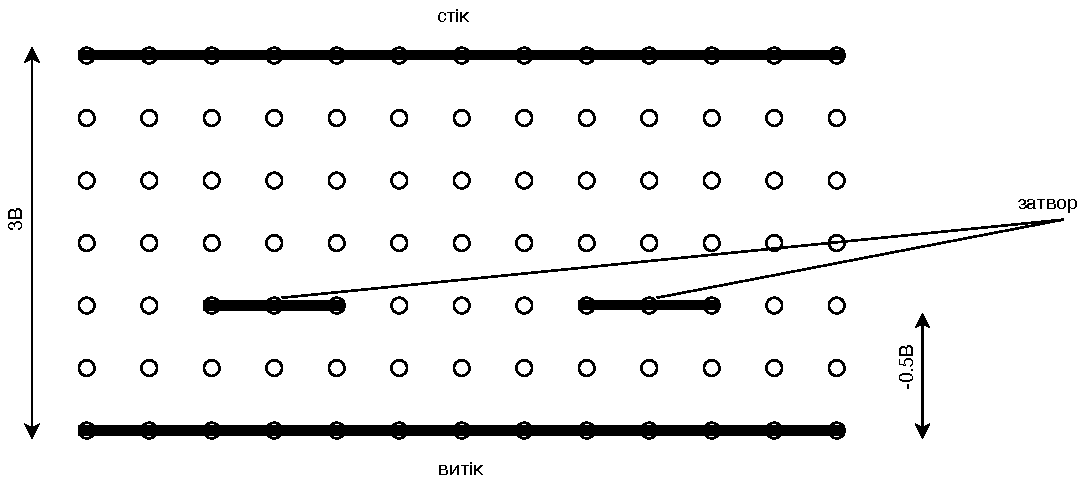
\includegraphics[width=1\linewidth]{0.pdf}}
\caption[wec]{Дисткретизація простору інтегрування за допомогою сітки з постійним кроком 0.5 мкм\footnotemark}
\label{ris:image}
\end{figure}
\footnotetext{Зауважимо, що для подальших розрахунків крок було зменшено вдвічі, тобто 0.25 мкм.}
\end{center}


При цьому двомірне рівняння Лапласа
\begin{equation}
\dfrac{\partial^2 V}{\partial x^2} +\dfrac{\partial^2 V}{\partial y^2} =0
\label{eq:ref}
\end{equation}
наближено заміняється наступним алгебраічним рівнянням:
\begin{equation}
V ( x + h, y ) + V ( x-h, y ) + V ( x, y + h ) + V ( x, y-h ) - 4 V ( x, y ) = 0
\label{eq:ref}
\end{equation}

\begin{landscape}

Спочатку програмно виведемо табл. \ref{tab:ref1} \text{ } нульового наближення, а також  табл.\ref{tab:ref2} \text{ } першого наближення.
\vspace{0.1cm}
\begin{center}
\tablecaption{ Нульове наближення}
\label{tab:ref1}
\begin{footnotesize}
\begin{supertabular}{| l| l| l| l| l| l| l| l| l| l| l| l| l| l| l| l| l| l| l| l| l| l| l| l| l| l| l| l|}
  \hline
  \csvreader[ separator=semicolon,late after line=\\\hline,]{data1.csv}{0=\Nr,1=\1,2=\2,3=\3,4=\4,5=\5,6=\6,7=\7,8=\8,9=\9,10=\a,11=\b,12=\c,13=\d,14=\e,15=\f,16=\g,17=\k,18=\o,19=\p,20=\r,21=\s,22=\t,23=\x,24=\y}
											{\Nr&\1&\2&\3&\4&\5&\6&\7&\8&\9&\a&\b&\c&\d&\f&\g&\k&\o&\r&\s&\t&\x&\y}
\end{supertabular}
 \end{footnotesize}


\vspace{2cm}

\tablecaption{Перше наближення}
\label{tab:ref2}
\begin{footnotesize}
\begin{supertabular}{| l| l| l| l| l| l| l| l| l| l| l| l| l| l| l| l| l| l| l| l| l| l| l| l| l| l| l| l|}
  \hline
  \csvreader[ separator=semicolon,late after line=\\\hline,]{data2.csv}{0=\Nr,1=\1,2=\2,3=\3,4=\4,5=\5,6=\6,7=\7,8=\8,9=\9,10=\a,11=\b,12=\c,13=\d,14=\e,15=\f,16=\g,17=\k,18=\o,19=\p,20=\r,21=\s,22=\t,23=\x,24=\y}
											{\Nr&\1&\2&\3&\4&\5&\6&\7&\8&\9&\a&\b&\c&\d&\f&\g&\k&\o&\r&\s&\t&\x&\y}
\end{supertabular}
 \end{footnotesize}
\end{center}



\newpage
Результат після 39 ітерацій:\\
\begin{center}
\vspace{0.2cm}
\label{tab:ref3}
\begin{footnotesize}
\tablecaption{Розподіл потенціалу в польовому транзисторі}
\begin{supertabular}{| l| l| l| l| l| l| l| l| l| l| l| l| l| l| l| l| l| l| l| l| l| l| l| l| l| l| l| l|}

  \hline
  \csvreader[ separator=semicolon,late after line=\\\hline,]{data.csv}{0=\Nr,1=\1,2=\2,3=\3,4=\4,5=\5,6=\6,7=\7,8=\8,9=\9,10=\a,11=\b,12=\c,13=\d,14=\e,15=\f,16=\g,17=\k,18=\o,19=\p,20=\r,21=\s,22=\t,23=\x,24=\y}
											{\Nr&\1&\2&\3&\4&\5&\6&\7&\8&\9&\a&\b&\c&\d&\f&\g&\k&\o&\r&\s&\t&\x&\y}


 \end{supertabular}
 \end{footnotesize}
\end{center}
 \end{landscape}
Візуалізація цих данних було наведено на Рис. \ref{ris:image1}, Рис. \ref{ris:image2}.


\begin{figure}[h]
\center{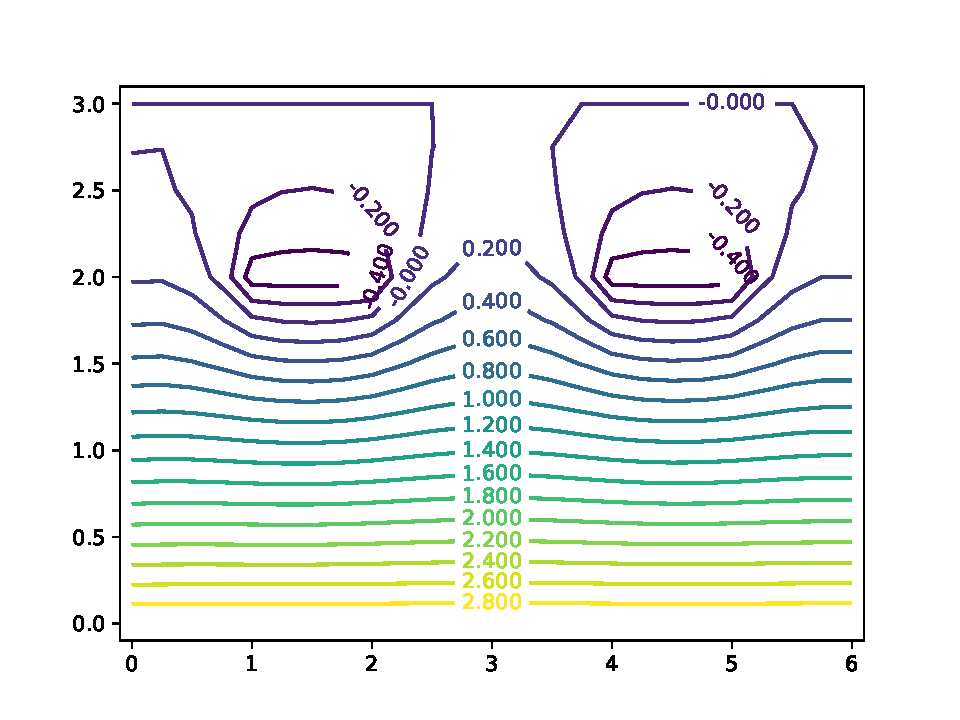
\includegraphics[width=1\linewidth]{2.pdf}}
\caption{Картина поля за допомогою еквіпотенціалей.}
\label{ris:image1}
\end{figure}

\begin{figure}
\center{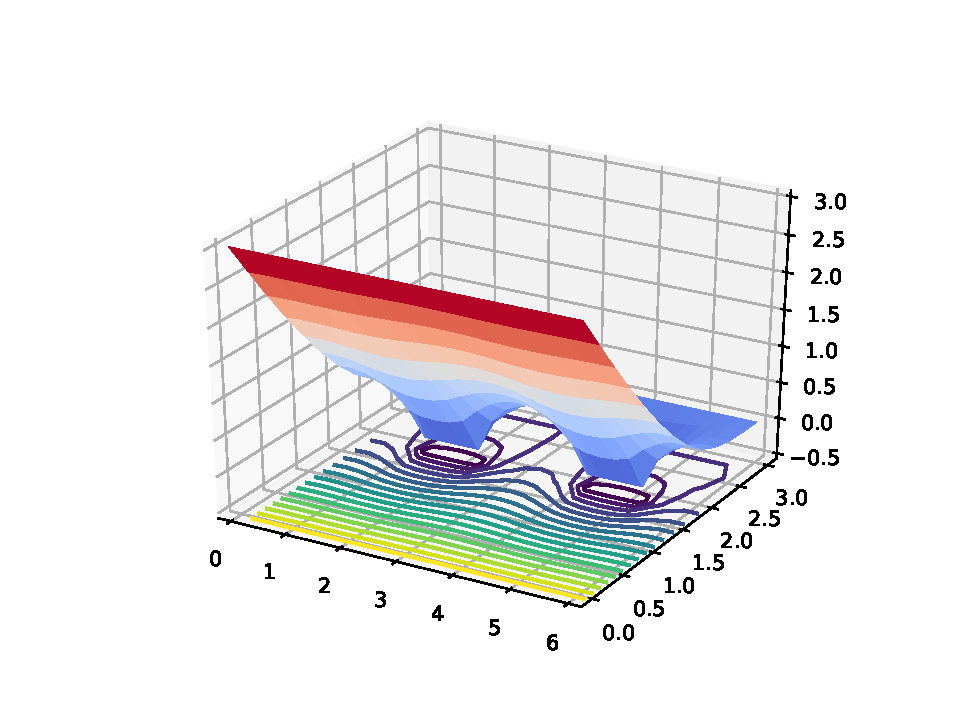
\includegraphics[width=1\linewidth]{3.pdf}}
\caption{Косокутна проекція потенціального рельєфу U(x,y).}
\label{ris:image2}
\end{figure}

\newpage

Розрахунок напруженості електричного поля провадиться за співвідношення $E_x$=$-\dfrac{\partial V}{\partial x}$, $E_y$=$\dfrac{\partial V}{\partial y}$що наближено обчислюються через кінцеві різниці. Використовуючи значення похідних зліва і справа, можна знайти середнє арифметичне
\begin{equation}
E_{x\text{ }i,j} = \dfrac{V_{(i-1),j}  + V_{(i+1),j}}{2}
\label{eq:ref}
\end{equation}
\begin{equation}
E_{y\text{ }i,j} = \dfrac{V_{i,(j-1)}  + V_{i,(j+1)}}{2}
\label{eq:ref}
\end{equation}











Наступним кроком я графічно зобразив веркори напруженості електричного поля в нашому польовому транзисторі (рис. \ref{ris:image3}). Дивлячись на цей рисунок можна чітко побачити що електричне поле яке прямує із стоку до затвору набагато сильніше ніж те що йде йому на зустріч, про що свідчать довжини стрілок.\\

\begin{center}
\begin{figure}[h]
\center{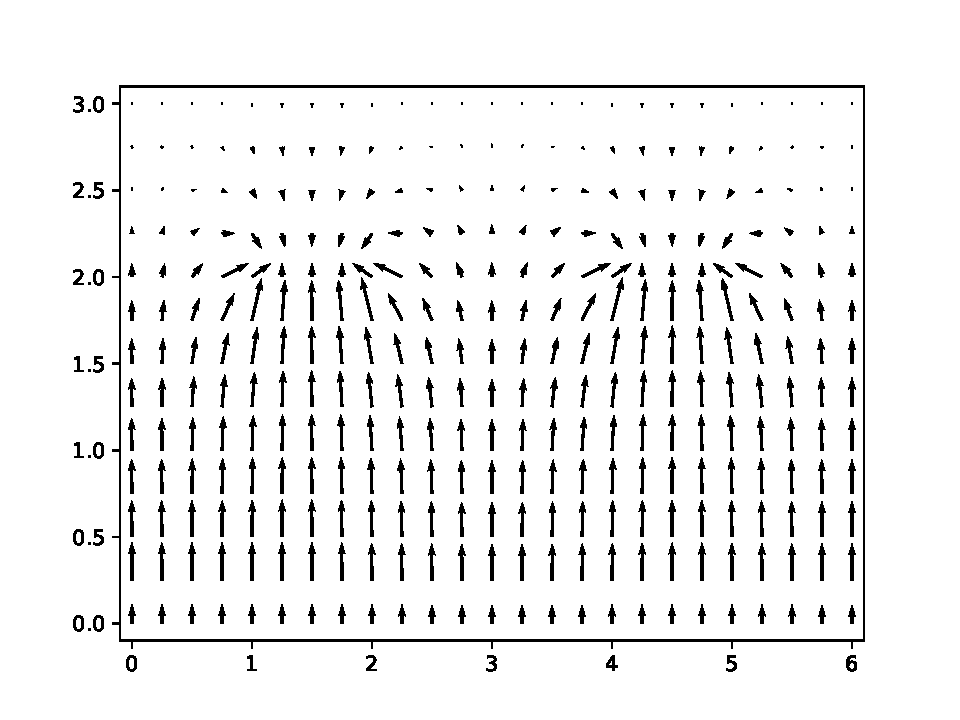
\includegraphics[width=1\linewidth]{1.pdf}}
\caption{Картина поля за допомогою векторів напруженості електричного поля.}
\label{ris:image3}
\end{figure}

\newpage
Останнім кроком я побудував косокутку проекцію потенціального рельєфу $U(x,y) = -eV(x,y)$ рис. \ref{ris:image4}
\begin{figure}[h]
\center{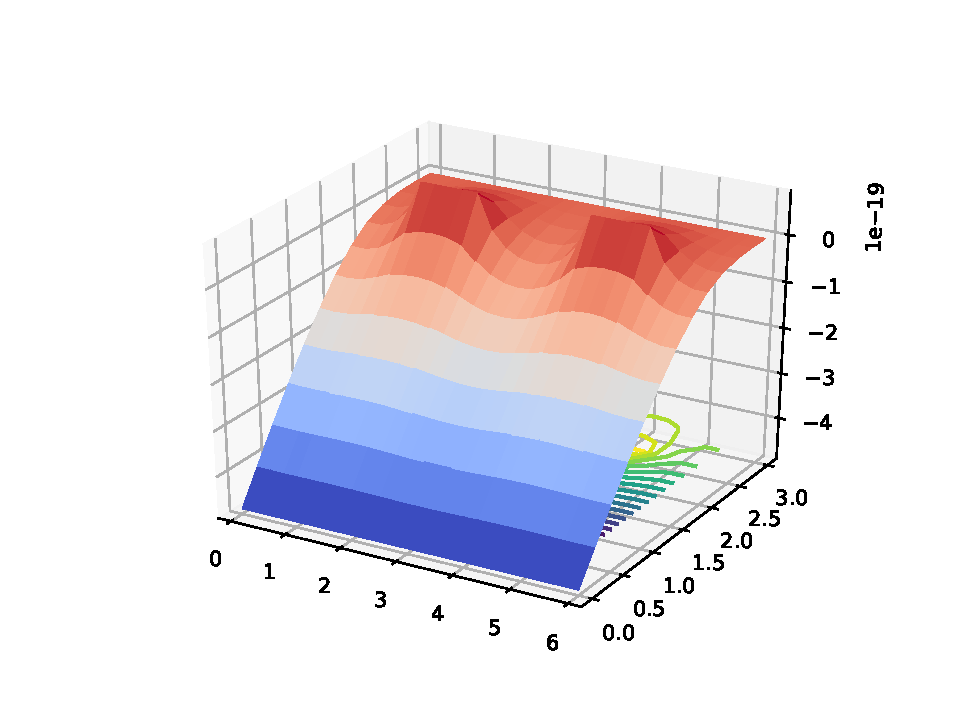
\includegraphics[width=1\linewidth]{3.1.pdf}}
\caption{Косокутна проекція потенціального рельєфу U(x,y) = -eV(x,y).}
\label{ris:image4}
\end{figure}
\end{center}







\clearpage
Висновок: \\

У цій розрахунковій роботі я засвоїв принципи та методи чисельного інтегрування рівнянь Лапласа, а також способи графічно зоображувати результати. Для визначення потенціалів дискретної сітки був застосований метод скінченних різниць, а також використані граничні умови Діріхле та Неймана. За допомогою ітераційного методу була досягнута задана в завданні точність 0.01В також були побудовані картини розподілу поля за допомогою еквіпотенціальних ліній та векторів напруженості електричного поля, а також була побудована косокутна проекція потенціального рельєфу. З отриманого графіка еквіпотенціалей помітні 2 ділянки, де є викривлення їх форми. Тут різко змінюється потенціал, оскільки це є затвор, на якому потенціал є постійним (в моєму випадку -0.5). При використанні векторів напруженості електричного поля, отримана картина покаже нам розподіл електричного поля в міжелектродному просторі. На отриманій же просторовій сітці, можемо побачити як вузли із розрахованим значенням потенціалу з’єднуються між собою прямими лініями, які і є еквіпотенціальними лініями.






\clearpage
\begin{center}
\textbf{ДОДАТОК}
\end{center}
Для обрахунку всіх значень, графіків та поверхонь я написав програму на мові Python:\\
\lstinputlisting[basicstyle=\ttfamily\footnotesize,language=Python]{rgr1.py}














\end{document}
